\documentclass[tikz,border=10pt]{standalone}
\usepackage{tkz-graph}
\usetikzlibrary{automata}
\usetikzlibrary[automata]
\begin{document}
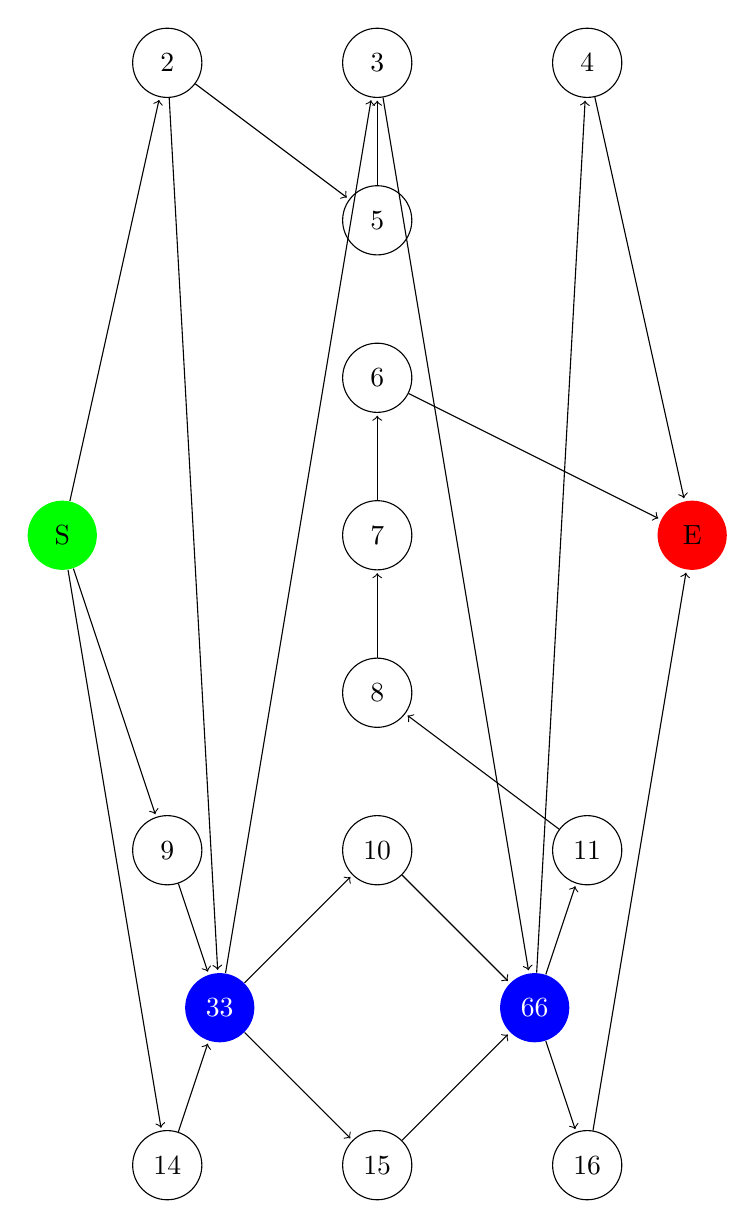
\begin{tikzpicture}[shorten >=1pt,node distance=3cm,auto,bend angle=45]
\node[state, fill,draw=none,green, text=black] (0) at (0,0) {S};
\node[state, fill,draw=none,red,text=black](1) at (8,0) {E};
\node[state] (2) at (1.33333,6) {$2$};
\node[state] (3) at (4,6) {$3$};
\node[state] (4) at (6.66667,6) {$4$};
\node[state] (5) at (4,4) {$5$};
\node[state] (6) at (4,2) {$6$};
\node[state] (7) at (4,0) {$7$};
\node[state] (8) at (4,-2) {$8$};
\node[state] (9) at (1.33333,-4) {$9$};
\node[state] (10) at (4,-4) {$10$};
\node[state] (11) at (6.66667,-4) {$11$};
\node[state, fill,draw=none,blue,text=white] (12) at (2,-6) {33};
\node[state, fill,draw=none,blue,text=white] (13) at (6,-6) {66};
\node[state] (14) at (1.33333,-8) {$14$};
\node[state] (15) at (4,-8) {$15$};
\node[state] (16) at (6.66667,-8) {$16$};
\path[->] 
(0) edge node {} (2)
(0) edge node {} (9)
(0) edge node {} (14)
(2) edge node {} (5)
(2) edge node {} (12)
(3) edge node {} (13)
(4) edge node {} (1)
(5) edge node {} (3)
(6) edge node {} (1)
(7) edge node {} (6)
(8) edge node {} (7)
(9) edge node {} (12)
(10) edge node {} (13)
(11) edge node {} (8)
(12) edge node {} (3)
(12) edge node {} (10)
(12) edge node {} (15)
(13) edge node {} (4)
(13) edge node {} (11)
(13) edge node {} (16)
(14) edge node {} (12)
(15) edge node {} (13)
(16) edge node {} (1)
;
\end{tikzpicture}
\end{document}
